\documentclass[../../main]{subfiles}
\begin{document}
\begin{figure}[h]

\begin{center}

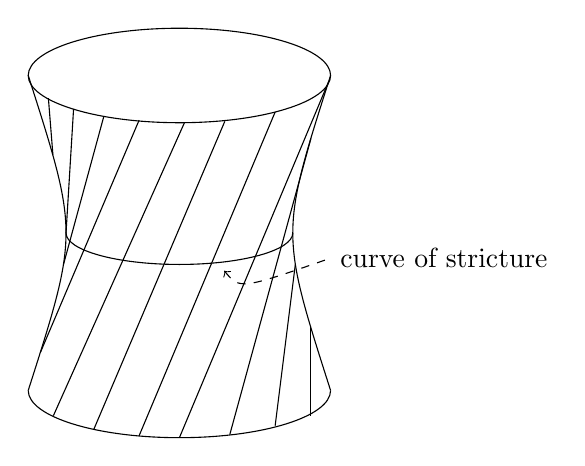
\begin{tikzpicture}[scale=.8, xscale=.8]
\draw (0,0) ellipse [x radius=3cm, y radius=.75cm];
\draw (3,-5) arc(0:-180:3cm and .75cm);
\draw (2.25,-2.5) arc(0:-180:2.25cm and .5cm);
\draw (3,0) .. controls (2,-2.5) and (2,-2.5) .. (3,-5);
\draw (-3,0) .. controls (-2,-2.5) and (-2,-2.5) .. (-3,-5);

%This should be done using coordinate.  But this works for now. -zxcvly

\draw (-2.6,-.36) -- (-2.51,-1.26);
\draw (-2.1,-.53) -- (-2.25,-2.5);
\draw (-1.5,-.65) -- (-2.3,-3);
\draw (-.8, -.71) -- (-2.76,-4.4);
\draw (.1,-.75) -- (-2.5,-5.4);
\draw (.9,-.73) -- (-1.7,-5.62);
\draw (1.9,-.58) -- (-.8,-5.72);
\draw (2.96,-.1) -- (0,-5.75);
\draw (2.61,-1) -- (1,-5.7);
\draw (2.3,-3) -- (1.9,-5.56);
\draw (2.6,-4) -- (2.6,-5.4);
\draw [dashed, <-] (.89, -3.1) .. controls (1.2,-3.4) .. (3,-2.9) node[anchor=west]{curve of stricture};

\end{tikzpicture}

\end{center}

\caption{Hyperboloid of Revolution}
\label{fig:ch02fig6}
\end{figure}

\end{document}